Dans un souci d'améliorer sa politique en matière de développement durable, une entreprise a réalisé une enquête statistique sur sa production de déchets.

Dans cette enquête, les déchets sont classés en trois catégories :

\begin{itemize}
	\item $69\,\%$ des déchets sont minéraux et non dangereux ;
	\item $28\,\%$ des déchets sont non minéraux et non dangereux ;
	\item les déchets restants sont des déchets dangereux.
\end{itemize}

Cette enquête statistique nous apprend également que :

\begin{itemize}
	\item $73$\,\% des déchets minéraux et non dangereux sont recyclables ;
	\item $49$\,\% des déchets non minéraux et non dangereux sont recyclables ;
	\item $35$\,\% des déchets dangereux sont recyclables.
\end{itemize}

\emph{Les parties A et B sont indépendantes et peuvent être traitées séparément.}

\medskip

\textbf{Partie A}

\medskip

Dans cette entreprise, on prélève au hasard un déchet. On considère les évènements suivants :

\begin{itemize}
	\item $M$ : \og Le déchet prélevé est minéral et non dangereux \fg{} ;
	\item $N$ : \og Le déchet prélevé est non minéral et non dangereux \fg{} ;
	\item $D$ : \og Le déchet prélevé est dangereux \fg{} ;
	\item $R$ : \og Le déchet prélevé est recyclable \fg.
\end{itemize}

On note $\overline{R}$ l'évènement contraire de l'évènement $R$.

\begin{enumerate}
	\item Recopier et compléter l'arbre pondéré ci-dessous représentant la situation de l'énoncé.
\end{enumerate}

\begin{center}
	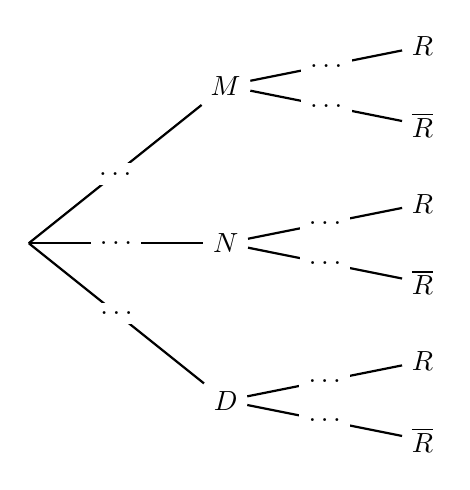
\begin{tikzpicture}
		\tikzstyle{fleche}=[thick]
		\tikzstyle{noeud}=[fill=white]
		\tikzstyle{etiquette}=[midway,fill=white]
		\def\DistanceInterNiveaux{2.5}
		\def\DistanceInterFeuilles{1}
		\def\NiveauA{(0)*\DistanceInterNiveaux}
		\def\NiveauB{(1)*\DistanceInterNiveaux}
		\def\NiveauC{(2)*\DistanceInterNiveaux}
		\def\InterFeuilles{(-1)*\DistanceInterFeuilles}
		\coordinate (R) at ({\NiveauA},{(2.5)*\InterFeuilles}) ;
		\node[noeud] (Ra) at ({\NiveauB},{(0.5)*\InterFeuilles}) {$M$};
		\node[noeud] (Raa) at ({\NiveauC},{(0)*\InterFeuilles}) {$R$};
		\node[noeud] (Rab) at ({\NiveauC},{(1)*\InterFeuilles}) {$\overline{R}$};
		\node[noeud] (Rb) at ({\NiveauB},{(2.5)*\InterFeuilles}) {$N$};
		\node[noeud] (Rba) at ({\NiveauC},{(2)*\InterFeuilles}) {$R$};
		\node[noeud] (Rbb) at ({\NiveauC},{(3)*\InterFeuilles}) {$\overline{R}$};
		\node[noeud] (Rc) at ({\NiveauB},{(4.5)*\InterFeuilles}) {$D$};
		\node[noeud] (Rca) at ({\NiveauC},{(4)*\InterFeuilles}) {$R$};
		\node[noeud] (Rcb) at ({\NiveauC},{(5)*\InterFeuilles}) {$\overline{R}$};
		\draw[fleche] (R)--(Ra) node[etiquette] {$\dots$};
		\draw[fleche] (Ra)--(Raa) node[etiquette] {$\dots$};
		\draw[fleche] (Ra)--(Rab) node[etiquette] {$\dots$};
		\draw[fleche] (R)--(Rb) node[etiquette] {$\dots$};
		\draw[fleche] (Rb)--(Rba) node[etiquette] {$\dots$};
		\draw[fleche] (Rb)--(Rbb) node[etiquette] {$\dots$};
		\draw[fleche] (R)--(Rc) node[etiquette] {$\dots$};
		\draw[fleche] (Rc)--(Rca) node[etiquette] {$\dots$};
		\draw[fleche] (Rc)--(Rcb) node[etiquette] {$\dots$};
	\end{tikzpicture}
\end{center}

\begin{enumerate}[resume]
	\item Justifier que la probabilité que le déchet soit dangereux et recyclable est égale à \num{0,0105}.
	\item Déterminer la probabilité $P\left(M \cap \overline{R}\right)$ et interpréter la réponse obtenue dans le contexte de l'exercice.
	\item Démontrer que la probabilité de l'évènement $R$ est $P(R)=\num{0,6514}$.
	\item On suppose que le déchet prélevé est recyclable. Déterminer la probabilité que ce déchet soit non minéral et non dangereux. \emph{On donnera la valeur arrondie au dix-millième.}
\end{enumerate}

\medskip

\textbf{Partie B}

\medskip

On rappelle que la probabilité qu'un déchet prélevé au hasard soit recyclable est égale à \num{0,6514}.

\begin{enumerate}
	\item Afin de contrôler la qualité de la collecte dans l'entreprise, on prélève un échantillon de 20 déchets pris au hasard dans la production. On suppose que le stock est suffisamment important pour assimiler le prélèvement de cet échantillon à un tirage avec remise.
	
	On désigne par $X$ la variable aléatoire égale au nombre de déchets recyclables dans cet échantillon.
	\begin{enumerate}
		\item On admet que la variable aléatoire $X$ suit une loi binomiale. Préciser ses paramètres.
		\item Donner la probabilité que l'échantillon contienne exactement 14 déchets recyclables. \emph{On donnera la valeur arrondie au dix-millième.}
	\end{enumerate}
	\item Dans cette question, on prélève désormais $n$ déchets, où $n$ désigne un entier naturel strictement positif.
	\begin{enumerate}
		\item Donner l'expression en fonction de $n$ de la probabilité $p_{n}$ qu'aucun déchet de cet échantillon ne soit recyclable.
		\item Déterminer la valeur de l'entier naturel $n$ à partir de laquelle la probabilité qu'au moins un déchet du prélèvement soit recyclable est supérieure ou égale à \num{0,9999}.
	\end{enumerate}
\end{enumerate}